\documentclass{exam}

\usepackage{lipsum} 
\usepackage[english]{babel}
\usepackage{amsmath}
\usepackage{amsfonts}
\usepackage{cancel}
\usepackage{pgfplots}
\usepackage{xcolor}
\usepackage{listings}
\usepackage{hyperref}
\usepackage{multirow}

\definecolor{codegreen}{rgb}{0,0.6,0}
\definecolor{codegray}{rgb}{0.5,0.5,0.5}
\definecolor{codepurple}{rgb}{0.58,0,0.82}
\definecolor{backcolour}{rgb}{0.95,0.95,0.92}

\lstdefinestyle{mystyle}{
    backgroundcolor=\color{backcolour},   
    commentstyle=\color{codegreen},
    keywordstyle=\color{magenta},
    numberstyle=\tiny\color{codegray},
    stringstyle=\color{codepurple},
    basicstyle=\ttfamily\footnotesize,
    breakatwhitespace=false,         
    breaklines=true,                 
    captionpos=b,                    
    keepspaces=true,                 
    numbers=left,                    
    numbersep=5pt,                  
    showspaces=false,                
    showstringspaces=false,
    showtabs=false,                  
    tabsize=2
}

\lstset{style=mystyle}


\begin{document}
\thispagestyle{plain}
\begin{titlepage}
    \begin{center}
        \vspace*{1cm}
            
        \Huge
        \textbf{The University of Hong Kong}
            
        \vspace{0.5cm}
        \LARGE
        COMP1117 Computer Programming
                     
        \vspace{0.4cm}
        \textbf{Exercise 2 Part B}

        \vspace{0.4cm}
        \textbf{Time allowed for both parts: 50 minutes}
        
        \begin{center}
        \fbox{\fbox{\parbox{5.5in}{\centering
        This paper is not written by any individuals from the Department of Computer Science. Please note that you are advised to do this paper with a pen and A4 paper. If you do not do that, the writer of this paper would be strongly disappointed :(}}}
        \end{center}
            
        \vfill
        \Large    
        Just a small tip: PLEASE do not use a debugger :P\\
        And no careless mistakes :(
            
        \vspace{0.8cm}
            
        \includegraphics[width=0.4\textwidth]{university}
            
        \Large
        Setter: Victor\\
        Last Updated: 2022-04-20
    \end{center}
\end{titlepage}
\begin{questions}
    \marksnotpoints 
    \question[15] In this question, you are going to write a program to select the words from a wordlist with most predefined alphabets. Given a wrost list $w = \{w_1, w_2, \ldots , w_n\}$ and a string of alphabet $s$, find the word(s) $w_x, \ldots, w_y$ in $w$, which contains most alphabetss found in $s$. The selection is case-insensitive. You may assume that the alphabets in s will not be repeated. Print the selected word(s) in ascending order. \\
    \begin{center}
    \begin{tabular}{ |p{1cm}||p{11cm}|p{2cm}|  }
    \hline
    \multicolumn{3}{|c|}{Sample Cases} \\
    \hline
    Case& Inputs & Outputs\\
    \hline
    \multirow{2}{4em}{1} & this is a test & is \\ 
& is & this \\ 
    \hline
    \multirow{2}{4em}{2} & There is nothing permanent except change & change \\
& Areing & \\
    \hline
    \multirow{2}{4em}{3} & moon river & river \\
& oie & \\
    \hline
    \end{tabular}
    \end{center}

    \question[15] Write a Python program that reads two numbers n and a from the console, and prints all the numbers from 1 to n which has exactly a factors excluding 1 and the number itself.
    \begin{center}
    \begin{tabular}{ |p{1cm}||p{11cm}|p{2cm}|  }
    \hline
    \multicolumn{3}{|c|}{Sample Cases} \\
    \hline
    Case& Inputs & Outputs\\
    \hline
    \multirow{2}{4em}{1} & 20 & 12 \\ 
& 4 & 18 \\ 
    \hline
    \multirow{2}{4em}{2} & 50 & 16 \\
& 3 & \\
    \hline
    \multirow{5}{4em}{3} & 20 & 1 \\
& 0 & 2\\
& & 3\\
& & 5\\
& & 7\\
    \hline
    \end{tabular}
    \end{center}
    
    \question[20] You are required to write a Python program which encrypts a plain text into a ciphertext (text after encryption) and decrypts a ciphertext into a plain text using the following codebook. During encryption, the program maps the letter in the first row to the corresponding letter in the second row. This process is reversed for decryption.\\
    For example:\\
    The ciphertext of "Hello" is "Qnssb". \\ 
    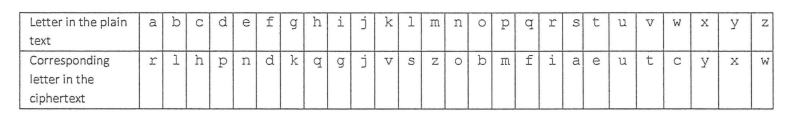
\includegraphics[width=15.0cm, scale=1.5]{photo} \\
    The first character of the input is either "e" or "d" followed by the message (without line break or space). If the first character is "e", the message should be encrypted, otherwise the message should be decrypted.
    \begin{center}
    \begin{tabular}{ |p{1cm}||p{11cm}|p{2cm}|  }
    \hline
    \multicolumn{3}{|c|}{Sample Cases} \\
    \hline
    Case& Inputs & Outputs\\
    \hline
    1 & eCOMP1117 & HBZM1117 \\ 
    \hline
    2 & eComputer Programming & this \\ 
    \hline
    3 & dNokgonnigok & Engineering \\
    \hline
    \end{tabular}
    \end{center}

    \end{questions} 
\end{document}
